\subsection{Constraints}
\label{app:constraints}

\begin{table}[H]
\centering
\caption{Constraints for Drone Design (Updated)}
\label{tab:constraints}
\begin{tabular}{|>{\centering\arraybackslash}p{0.05\textwidth} | >{\centering\arraybackslash}p{0.13\textwidth} | p{0.42\textwidth} | p{0.30\textwidth}|}
\hline
\rowcolor{gray!15}
\textbf{No.} & \textbf{Constraint} & \textbf{Description} & \textbf{Assumptions} \\
\hline
C.1 & Weight & The total weight of the drone must allow for continuous and stable flight. & The quad-mounted motors can support a maximum payload of 60\,g. \\
\hline
C.2 & Software & Only free and open-source flight controller software shall be used. & The firmware will incorporate third-party open-source code, which will be modified to suit the application (e.g., autonomy and feedback). \\
\hline
C.3 & Operating Environment & The drone is limited to operation within a fixed indoor area containing immovable fixtures (e.g., wall-mounted displays). & -- \\
\hline
C.4 & Budget & The design and construction of the drone shall remain within the allocated project budget. & -- \\
\hline
C.5 & Network Speed & Wireless bandwidth and latency may limit the system’s ability to stream live video. & Streaming will occur via \gls{uwa} Wi-Fi or a mobile hotspot. \\
\hline
C.6 & Safety & The drone must be safe for operation by the user and must not pose any physical risk to personnel. & -- \\
\hline
C.7 & Sensor Selection & Available sensors (such as \gls{imu} and \gls{tof}) are constrained by cost, availability, and ability to interface with the ESP32 microcontroller. & Supported interfaces include \gls{uart}, \gls{i2c}, and \gls{spi}. \\
\hline
\end{tabular}
\end{table}

\subsection{Additional Requirements}
\label{app:additional_req}

\begin{table}[H]
\centering
\caption{Additional Requirements}
\begin{tabular}{|>{\centering\arraybackslash}p{0.1\textwidth} | p{0.8\textwidth}|}
\hline
\rowcolor{gray!15}
\textbf{No.} & \textbf{Requirement} \\
\hline
R.16 & The \gls{pcb} shall include custom motor drivers. \\
\hline
R.19 & The drone shall be able to fly for a minimum of 3 minutes. \\
\hline
R.28 & The surveillance camera shall stream a live camera feed. \\
\hline
R.26 & The UI shall include a battery level monitoring system for detecting low battery levels. \\
\hline
R.29 & The surveillance camera shall record video for playback. \\
\hline
R.25 & The UI shall include an error diagnostic and feedback system. \\
\hline
R.6  & The hovering altitude shall be adjustable prior to operation, within a range of 0.5 to 2 metres. \\
\hline
A.R.2 & The drone’s operational capabilities shall be powered by a single battery. \\
\hline
A.R.4 & A comprehensive operation manual and user guide shall be provided to the client for use, understanding, and further development. \\
\hline
A.R.6 & Placement of components on the \gls{pcb} shall minimise signal distortion and heat generation to ensure accurate flight paths and predictable behaviour. \\
\hline
A.R.7 & The drone shall feature a visual (LED) or audible warning system to alert personnel during flight initiation. \\
\hline
A.R.8 & The drone shall provide a UI alert in cases of overheating. \\
\hline
A.R.9 & The drone shall include LEDs to indicate charging mode. \\
\hline
A.R.10 & The drone shall feature visual or UI indicators showing when it is powering down or operating autonomously. \\
\hline
\end{tabular}
\end{table}

%----------------------------------------------------------%
\subsection{WebSocket}
\label{app:websocket}

\begin{figure}[H]
    \centering
    \captionsetup{justification=centering, margin=1cm}
    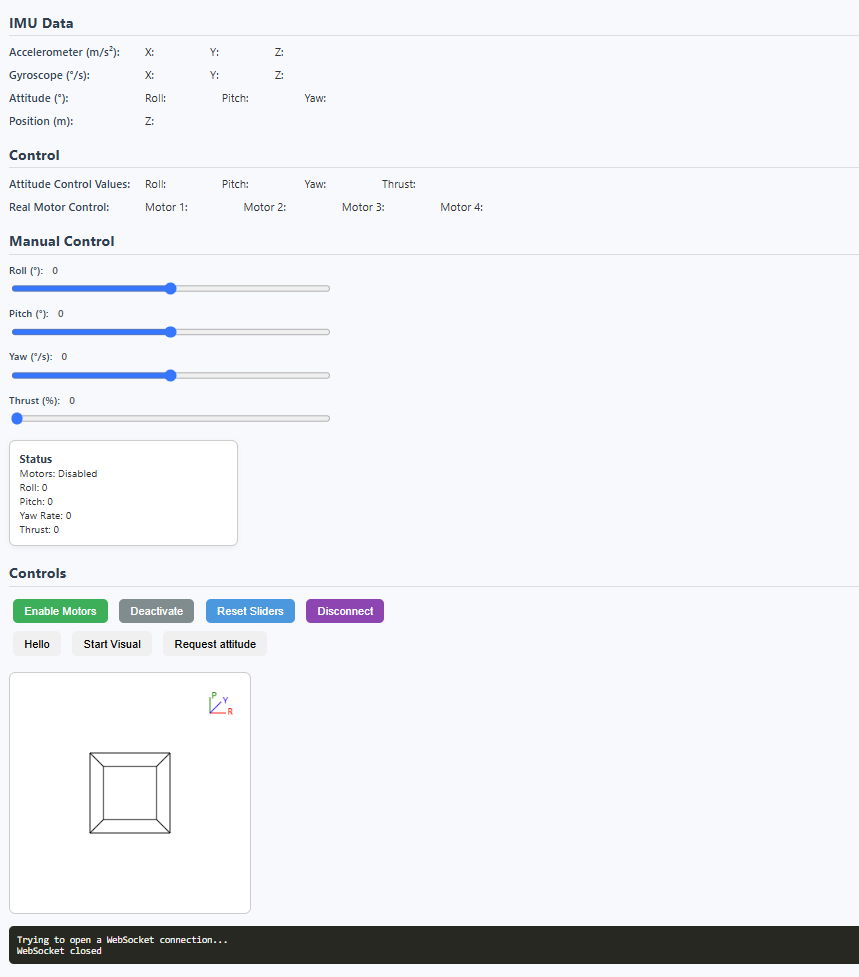
\includegraphics[width=0.55\textwidth]{img/websocket-page.PNG}
    \caption{WebSocket Client Web Page}
\end{figure}

%----------------------------------------------------------%
\pagebreak

\subsection{Requirements Update Summary (Week 6)}
\label{app:req-changes}

\subsubsection{Ranked Requirements - Proposed Changes}

\begin{table}[H]
\centering
\caption{Ranked Requirements Proposed Changes}
\begin{tabular}{|c|c|p{11cm}|}
\hline
\textbf{Rank} & \textbf{No.} & \textbf{Requirement Description} \\ \hline
1 & R.2 & The drone shall be capable of hovering and flying. \\ \hline
2 & R.30 & The drone must power off after 30s of disconnection. \\ \hline
3 & R.1 & The drone shall operate in an indoor area. \\ \hline
4 & R.17 & The drone shall utilise shrouded propellers or dedicated propeller guards. \\ \hline
5 & R.3 & The drone shall navigate without the use of GPS. \\ \hline
6 & R.4 & The drone shall maintain a set hovering altitude during autonomous surveillance. \\ \hline
7 & R.14 & A manual override system shall be available to the user. \\ \hline
8 & R.27 & The drone shall autonomously land safely when battery levels are low. \\ \hline
9 & R.24 & Any third-party software used for the drone control system must be open-source and freely available. \\ \hline
10 & R.7 & \textcolor{red}{\sout{The drone shall be able to navigate autonomously.}} \\ \hline
11 & R.11 & \textcolor{red}{\sout{The drone should be capable of detecting obstacles.}} \\ \hline
12 & R.12 & \textcolor{red}{\sout{The drone shall be capable of avoiding non-transparent obstacles (including walls) by stopping and hovering.}} \\ \hline
13 & R.23 & The drone design shall remain within a budget of \$350.00. \\ \hline
14 & R.20 & The drone shall be capable of flight stabilisation. \\ \hline
15 & R.5 & The drone shall maintain a default altitude of 1.2-1.3 metres above ground level while surveying an area. \\ \hline
16 & R.18 & The power supplied shall be via one 1S or 2S Li-Po battery with a capacity up to 800mAh. \\ \hline
17 & R.15 & The drone shall have a custom PCB design for the flight controller which includes sensors and power distribution. \\ \hline
18 & R.8 & \textcolor{red}{\sout{The drone shall follow a predefined path set before beginning operation.}} \\ \hline
19 & R.13 & \textcolor{red}{\sout{The drone shall power down if it detects an obstacle and the obstacle is not removed within a certain time limit.}} \\ \hline
20 & R.21 & The drone shall maintain stability under wind conditions and disturbances. \\ \hline
\end{tabular}
\end{table}

\begin{table}[H]
\centering
\caption{Ranked Requirements - Final}
\begin{tabular}{|c|c|p{11cm}|}
\hline
\textbf{Rank} & \textbf{No.} & \textbf{Requirement Description} \\ \hline
1 & R.2 & The drone shall be capable of hovering and flying. \\ \hline
2 & R.30 & The drone must power off after 30s of disconnection. \\ \hline
3 & R.1 & The drone shall operate in an indoor area. \\ \hline
4 & R.17 & The drone shall utilise shrouded propellers or dedicated propeller guards. \\ \hline
5 & R.3 & The drone shall navigate without the use of GPS. \\ \hline
6 & R.4 & The drone shall maintain a set hovering altitude during autonomous surveillance. \\ \hline
7 & R.14 & A manual override system shall be available to the user. \\ \hline
8 & R.27 & The drone shall autonomously land safely when battery levels are low. \\ \hline
9 & R.24 & Any third-party software used for the drone control system must be open-source and freely available. \\ \hline
10 & R.23 & The drone design shall remain within a budget of \$350.00. \\ \hline
11 & R.20 & The drone shall be capable of flight stabilisation. \\ \hline
12 & R.5 & The drone shall maintain a default altitude of 1.2-1.3 metres above ground level while surveying an area. \\ \hline
13 & R.18 & The power supplied shall be via one 1S or 2S Li-Po battery with a capacity up to 800mAh. \\ \hline
14 & R.15 & The drone shall have a custom PCB design for the flight controller which includes sensors and power distribution. \\ \hline
15 & R.21 & The drone shall maintain stability under wind conditions and disturbances. \\ \hline
\end{tabular}
\end{table}

\subsubsection{Additional Requirements - Proposed Changes}

\begin{table}[H]
\centering
\caption{Additional Requirements Proposed Changes}
\begin{tabular}{|c|p{11cm}|}
\hline
\textbf{No.} & \textbf{Description} \\ \hline
R.16 & The PCB shall include custom motor drivers. \\ \hline
R.19 & The drone shall be able to fly for a minimum of 3 minutes. \\ \hline
R.28 & The surveillance camera shall stream the live camera feed. \\ \hline
R.9 & \textcolor{red}{\sout{There shall be a predefined set of options for the drone flight.}} \\ \hline
R.26 & The UI shall have a battery level monitoring system available for low battery levels. \\ \hline
R.29 & The surveillance camera shall record video for playback. \\ \hline
R.25 & The UI shall have an error diagnostic and feedback system. \\ \hline
R.6 & The hovering altitude shall be adjustable prior to operation (between 0.5 and 2 metres). \\ \hline
R.10 & \textcolor{red}{\sout{There shall be the option to change the predefined flight pattern to a custom option.}} \\ \hline
A.R.1 & \textcolor{red}{\sout{Pre-defined flight path shall follow a polygonal pattern of fixed altitude.}} \\ \hline
A.R.2 & The required drone operational capabilities shall be powered with only one battery. \\ \hline
A.R.3 & \textcolor{red}{\sout{When an obstacle is detected, the drone shall stop and hover until the obstacle is removed or a timeout occurs.}} \\ \hline
A.R.4 & A comprehensive operation manual and user guide shall be provided to the client. \\ \hline
A.R.5 & \textcolor{red}{\sout{The pre-determined flight path shape shall be adjustable in size.}} \\ \hline
A.R.6 & Placement of PCB components shall minimise signal distortion and heating. \\ \hline
A.R.7 & The drone shall have a visual or audible indication during initiation of flight. \\ \hline
A.R.8 & The drone shall alert on the UI in cases of overheating. \\ \hline
A.R.9 & The drone shall have LEDs to show when it is in charging mode. \\ \hline
A.R.10 & The drone shall have indicators to show when it is powering down or operating autonomously. \\ \hline
\end{tabular}
\end{table}

\subsubsection{Additional Requirements - Final (Post-Change List)}

\begin{table}[H]
\centering
\caption{Additional Requirements - Final}
\begin{tabular}{|c|p{11cm}|}
\hline
\textbf{No.} & \textbf{Description} \\ \hline
R.16 & The PCB shall include custom motor drivers. \\ \hline
R.19 & The drone shall be able to fly for a minimum of 3 minutes. \\ \hline
R.28 & The surveillance camera shall stream the live camera feed. \\ \hline
R.26 & The UI shall have a battery level monitoring system for low battery levels. \\ \hline
R.29 & The surveillance camera shall record video for playback. \\ \hline
R.25 & The UI shall have an error diagnostic and feedback system. \\ \hline
R.6 & The hovering altitude shall be adjustable prior to operation (between 0.5 and 2 metres). \\ \hline
A.R.2 & The required drone operational capabilities shall be powered with only one battery. \\ \hline
A.R.4 & A comprehensive operation manual and user guide shall be provided to the client. \\ \hline
A.R.6 & Placement of PCB components shall minimise signal distortion and heating. \\ \hline
A.R.7 & The drone shall have a visual or audible indication during initiation of flight. \\ \hline
A.R.8 & The drone shall alert on the UI in cases of overheating. \\ \hline
A.R.9 & The drone shall have LEDs to show when it is in charging mode. \\ \hline
A.R.10 & The drone shall have indicators to show when it is powering down or operating autonomously. \\ \hline
\end{tabular}
\end{table}

\textbf{Legend:}  
\textcolor{red}{\sout{Removed}} = Requirement removed in final approved version due to scope or redundancy.
%-------------------------------------------%
\pagebreak
\subsection{Code}
\subsubsection{sensor.c}
\label{app:sensor-code}

\begin{lstlisting}[caption={Register Read}]
//Ref: https://github.com/hibit-dev/mpu6050
//Ref: https://components.espressif.com/components/espressif/mpu6050

#include "i2c.h"
#include "stabiliser.h"
#include "sensors.h"
#include "filter.c"

#define MPU6050_SENSOR_ADDR         0x68
#define MPU6050_WHO_AM_I_REG_ADDR   0x75
#define MPU6050_ACCEL_XOUT_H_ADDR   0x3b 
#define MPU6050_GYRO_XOUT_H_ADDR    0x43
#define MPU6050_PWR_MGMT_1_ADDR     0x6b 
#define MPU6050_GYRO_CONFIG_ADDR    0x1b
#define MPU6050_ACCEL_CONFIG_ADDR   0x1c
#define MPU6050_INT_CFG_ADDR        0x37
#define MPU6050_INT_ENABLE_ADDR     0x38
#define MPU6050_DLPF_ADDR           0x1a
#define MPU6050_H_RESET             0x80
#define MPU6050_SLV4_CTRL_ADDR      0x34
#define MPU6050_MAST_CTRL_ADDR      0x24
#define MPU6050_SMPLRT_DIV_ADDR     0x19

#define GYRO_FULL_SCALE_250_DPS  0x00
#define GYRO_FULL_SCALE_500_DPS  0x08
#define GYRO_FULL_SCALE_1000_DPS 0x10
#define GYRO_FULL_SCALE_2000_DPS 0x18
#define ACC_FULL_SCALE_2G        0x00
#define ACC_FULL_SCALE_4G        0x08
#define ACC_FULL_SCALE_8G        0x10
#define ACC_FULL_SCALE_16G       0x18

#define GYRO_250_SENSITIVITY    (float)((2 * 250.0) / 65536.0)
#define GYRO_500_SENSITIVITY    (float)((2 * 500.0) / 65536.0)
#define GYRO_1000_SENSITIVITY   (float)((2 * 1000.0) / 65536.0)
#define GYRO_2000_SENSITIVITY   (float)((2 * 2000.0) / 65536.0)
#define ACC_2G_SENSITIVITY      (float)((2 * 2) / 65536.0)
#define ACC_4G_SENSITIVITY      (float)((2 * 4) / 65536.0)
#define ACC_8G_SENSITIVITY      (float)((2 * 8) / 65536.0)
#define ACC_16G_SENSITIVITY     (float)((2 * 16) / 65536.0)

#define GYRO_LPF_CUTOFF_FREQ 80
#define ACCE_LPF_CUTOFF_FREQ 30

/* The sensitivity must match the range: */
#define GYRO_SENSITIVITY GYRO_500_SENSITIVITY
#define ACCE_SENSITIVITY ACC_8G_SENSITIVITY
#define GYRO_CONFIG_RANGE GYRO_FULL_SCALE_500_DPS
#define ACCE_CONFIG_RANGE ACC_FULL_SCALE_8G

#define CALIBRATION_SAMPLES 200
#define INT_EN 1
bool use_bias = true;

static const char *TAG = "IMU";

QueueHandle_t acce_queue = NULL;
QueueHandle_t gyro_queue = NULL;
static TaskHandle_t sensor_task_handle = NULL;

static SemaphoreHandle_t mpu6050_data_ready;
static SemaphoreHandle_t sensor_data_ready;

static i2c_master_bus_handle_t bus_handle;
static i2c_master_dev_handle_t dev_handle;
static raw_acce_t raw_acce; 
static raw_gyro_t raw_gyro;
static gyro_t gyro;
static acce_t acce;
static raw_gyro_t gyro_bias = {.x = 0, .y = 0, .z = 0};
static raw_acce_t acce_bias = {.x = 0, .y = 0, .z = 0};

static lpf_data lpf_data_acce[3];
static lpf_data lpf_data_gyro[3];

static bool sensors_init = false;

/* INIT *****************************************************************/
esp_err_t mpu6050_init(i2c_master_bus_handle_t *bus_handle, i2c_master_dev_handle_t *dev_handle) {
    // Intialise the I2C master and device
    i2c_master_init(bus_handle, dev_handle);
    i2c_mpu_device_init(bus_handle, dev_handle);

    ESP_LOGI(TAG, "I2C initialized successfully");
    vTaskDelay(pdMS_TO_TICKS(100)); 
    
    // Reset the registers
    ESP_ERROR_CHECK(mpu6050_register_write_byte(*dev_handle, MPU6050_PWR_MGMT_1_ADDR, MPU6050_H_RESET));
    vTaskDelay(pdMS_TO_TICKS(100)); 
    
    // Set the gyro as the reference
    ESP_ERROR_CHECK(mpu6050_register_write_byte(*dev_handle, MPU6050_PWR_MGMT_1_ADDR, 0x01));

    uint8_t data[2];
    esp_err_t ret = mpu6050_register_read(*dev_handle, MPU6050_WHO_AM_I_REG_ADDR, data, 0x01);
    if (ret != ESP_OK || data[0] != 0x68) return 1;
        
    // Configure the sensor sensitivity
    ESP_ERROR_CHECK(mpu6050_register_write_byte(*dev_handle, MPU6050_ACCEL_CONFIG_ADDR, ACCE_CONFIG_RANGE));
    ESP_ERROR_CHECK(mpu6050_register_write_byte(*dev_handle, MPU6050_GYRO_CONFIG_ADDR, GYRO_CONFIG_RANGE));

    // Enable digital low pass (reduces sample rate from 8kHz to 1kHz)
    ESP_ERROR_CHECK(mpu6050_register_write_byte(*dev_handle, MPU6050_DLPF_ADDR, 0x02)); // 98Hz BW
    ESP_ERROR_CHECK(mpu6050_register_write_byte(*dev_handle, MPU6050_SMPLRT_DIV_ADDR, 0));

    // Enable interrupts
    ESP_ERROR_CHECK(mpu6050_register_write_byte(*dev_handle, MPU6050_INT_ENABLE_ADDR, INT_EN));
    ESP_ERROR_CHECK(mpu6050_register_write_byte(*dev_handle, MPU6050_INT_CFG_ADDR, 0x00));

    // Wake up the IMU
    ESP_ERROR_CHECK(mpu6050_register_write_byte(*dev_handle, MPU6050_PWR_MGMT_1_ADDR, 0x00));
    vTaskDelay(pdMS_TO_TICKS(100)); 

    return ESP_OK;
}

/* De-initialise IMU */
void mpu6050_deinit(i2c_master_bus_handle_t *bus_handle, i2c_master_dev_handle_t *dev_handle) {
    i2c_master_bus_rm_device(*dev_handle);
    i2c_del_master_bus(*bus_handle);
    ESP_LOGI(TAG, "I2C de-initialized successfully");
}

/* MOTION ******************************************************************/
/* Read MPU6050 acceleration */
void mpu6050_read_motion_acce(i2c_master_dev_handle_t *dev_handle, raw_acce_t *raw_acce, acce_t *acce, lpf_data *lpf_data) {
    // Registers (dec):
    // [59-64] Accelerometer

    uint8_t buffer[6];
    esp_err_t ret = mpu6050_register_read(*dev_handle, MPU6050_ACCEL_XOUT_H_ADDR, buffer, sizeof(buffer));

    if (ret != ESP_OK) {
        ESP_LOGE(TAG, "Failed to read from accelerometer");
        return;
    }
    
    raw_acce->x = (((int16_t) buffer[0]) << 8) | buffer[1];
    raw_acce->y = (((int16_t) buffer[2]) << 8) | buffer[3];
    raw_acce->z = (((int16_t) buffer[4]) << 8) | buffer[5];
    
    float x, y, z; 
    x = ((float)(raw_acce->x)) * ACCE_SENSITIVITY;
    y = ((float)(raw_acce->y)) * ACCE_SENSITIVITY;
    z = ((float)(raw_acce->z)) * ACCE_SENSITIVITY;

    acce->x = apply_lpf(&lpf_data[0], x);
    acce->y = apply_lpf(&lpf_data[1], y);
    acce->z = apply_lpf(&lpf_data[2], z);
}

/* Read MPU6050 gyroscope */
void mpu6050_read_motion_gyro(i2c_master_dev_handle_t *dev_handle, raw_gyro_t *raw_gyro, gyro_t *gyro,
                              raw_gyro_t *gyro_bias, lpf_data *lpf_data) {
    // Registers (dec):
    // [67-72] Gyroscope
    uint8_t buffer[6];
    esp_err_t ret = mpu6050_register_read(*dev_handle, MPU6050_GYRO_XOUT_H_ADDR, buffer, sizeof(buffer));
    if (ret != ESP_OK) {
        ESP_LOGE(TAG, "Failed to read from gyro");
        return;
    }

    raw_gyro->x = (((int16_t) buffer[0]) << 8) | buffer[1];
    raw_gyro->y = (((int16_t) buffer[2]) << 8) | buffer[3];
    raw_gyro->z = (((int16_t) buffer[4]) << 8) | buffer[5];
    
    float x, y, z; 
    x = ((float)(raw_gyro->x - gyro_bias->x)) * GYRO_SENSITIVITY;
    y = ((float)(raw_gyro->y - gyro_bias->y)) * GYRO_SENSITIVITY;
    z = ((float)(raw_gyro->z - gyro_bias->z)) * GYRO_SENSITIVITY;

    gyro->x = apply_lpf(&lpf_data[0], x);
    gyro->y = apply_lpf(&lpf_data[1], y);
    gyro->z = apply_lpf(&lpf_data[2], z);
}

void mpu6050_read_motion_raw(i2c_master_dev_handle_t *dev_handle, raw_gyro_t *raw_gyro, raw_acce_t *raw_acce) {
    uint8_t buffer[14];
    mpu6050_register_read(*dev_handle, MPU6050_GYRO_XOUT_H_ADDR, buffer, sizeof(buffer));

    raw_gyro->x = (((int16_t) buffer[0]) << 8) | buffer[1];
    raw_gyro->y = (((int16_t) buffer[2]) << 8) | buffer[3];
    raw_gyro->z = (((int16_t) buffer[4]) << 8) | buffer[5];
    raw_acce->x = (((int16_t) buffer[8]) << 8) | buffer[9];
    raw_acce->y = (((int16_t) buffer[10]) << 8) | buffer[11];
    raw_acce->z = (((int16_t) buffer[12]) << 8) | buffer[13];
}

/* Calibration *************************************************************/
void mpu6050_calibrate(i2c_master_dev_handle_t *dev_handle, raw_gyro_t *raw_gyro, raw_acce_t *raw_acce, raw_gyro_t *gyro_bias, raw_acce_t *acce_bias) {
    uint16_t samples = CALIBRATION_SAMPLES;
    int64_t g_sum_x = 0, g_sum_y = 0, g_sum_z = 0, a_sum_x = 0, a_sum_y = 0, a_sum_z = 0;

    for (int i = 0; i < samples; i++) {
        mpu6050_read_motion_raw(dev_handle, raw_gyro, raw_acce);
        g_sum_x += raw_gyro->x;
        g_sum_y += raw_gyro->y;
        g_sum_z += raw_gyro->z;
        vTaskDelay(pdMS_TO_TICKS(10)); 
    }

    gyro_bias->x = g_sum_x/samples;
    gyro_bias->y = g_sum_y/samples;
    gyro_bias->z = g_sum_z/samples;

    ESP_LOGI(TAG, "Gyro calibrated!");

    ESP_LOGI(TAG, "Gyro Bias: Gx: %.4f Gy: %.4f Gz: %.4f",
        (float)(gyro_bias->x) * GYRO_SENSITIVITY,
        (float)(gyro_bias->y) * GYRO_SENSITIVITY,
        (float)(gyro_bias->z) * GYRO_SENSITIVITY);
}

/**************************************************************/
/* Signal when data is ready from MPU6050 */
void IRAM_ATTR sensorISRHandler(void *arg) {
    // See: FreeRTOS website, xSemaphoreGiveFromISR()
    portBASE_TYPE xHigherPriorityTaskWoken = pdFALSE;
    xSemaphoreGiveFromISR(mpu6050_data_ready, &xHigherPriorityTaskWoken);

    if (xHigherPriorityTaskWoken) {
        portYIELD_FROM_ISR();
    }
}

/* Task *************************************************************/
static void sensor_task(void *arg) {
    // ESP_LOGI(TAG, "Ready to read from mpu6050...");
    while (1) {
        if ((xSemaphoreTake(mpu6050_data_ready, portMAX_DELAY) == pdTRUE)) {
        mpu6050_read_motion_acce(&dev_handle, &raw_acce, &acce, lpf_data_acce);
        xQueueOverwrite(acce_queue, (void *)&acce);

        mpu6050_read_motion_gyro(&dev_handle, &raw_gyro, &gyro, &gyro_bias, lpf_data_gyro);
        xQueueOverwrite(gyro_queue, (void *)&gyro);

        xSemaphoreGive(sensor_data_ready); 
        }
    }
}

void sensor_task_init(void) {
    acce_queue = xQueueCreate(1, sizeof(acce_t));
    gyro_queue = xQueueCreate(1, sizeof(gyro_t));
    mpu6050_data_ready = xSemaphoreCreateBinary();
    sensor_data_ready = xSemaphoreCreateBinary();

    esp_err_t ret = mpu6050_init(&bus_handle, &dev_handle);
    if (ret != ESP_OK) {
        ESP_LOGE(TAG, "Sensor not present or couldn't be read from");
        return;
    }
    vTaskDelay(pdMS_TO_TICKS(100)); 

    if (use_bias) mpu6050_calibrate(&dev_handle, &raw_gyro, &raw_acce, &gyro_bias, &acce_bias);

    for (uint8_t i = 0; i < 3; i++) {
        init_lpf(&lpf_data_acce[i], 1000.0, ACCE_LPF_CUTOFF_FREQ);
        init_lpf(&lpf_data_gyro[i], 1000.0, GYRO_LPF_CUTOFF_FREQ);
    }

    /* Configure interrupt pin */
    gpio_config_t io_conf = {
        .intr_type = GPIO_INTR_POSEDGE, // interrupt of rising edge
        .pin_bit_mask = (1ULL << MPU6050_INT_GPIO_PIN), // bit mask map of the pins for esp
        .mode = GPIO_MODE_INPUT, // set as input mode
        .pull_down_en = 0, // disable pull-down mode
        .pull_up_en = 1, // enable pull-up mode
    };
    
    gpio_config(&io_conf);
    gpio_install_isr_service(0);
    gpio_set_intr_type(MPU6050_INT_GPIO_PIN, GPIO_INTR_POSEDGE);
    gpio_isr_handler_add(MPU6050_INT_GPIO_PIN, sensorISRHandler, (void *)MPU6050_INT_GPIO_PIN);

    ESP_LOGI(TAG, "Sensor interrupt intialised");
    vTaskDelay(pdMS_TO_TICKS(100)); 

    /* Start the task */
    xTaskCreate(sensor_task, "sensor task", 2*1024, NULL, 1, &sensor_task_handle);
    ESP_LOGI(TAG, "Sensor task intialised");
    sensors_init = true; 
}

/**************************************************************/
/* Functions to interface with other tasks */
void waitSensorData() { 
    xSemaphoreTake(sensor_data_ready, portMAX_DELAY);
}

bool sensorsIsInit(void) {
    return sensors_init;
}

void readIMUData(sensor_data_t *sensor_data) {
    xQueuePeek(gyro_queue, (void *)&(sensor_data->gyro), 0);
    xQueuePeek(acce_queue, (void *)&(sensor_data->acce), 0);
}

/**************************************************************/

/* Read from MPU6050 register */
esp_err_t mpu6050_register_read(i2c_master_dev_handle_t dev_handle, uint8_t reg_addr, uint8_t *data, size_t len) {
    return i2c_master_transmit_receive(dev_handle, &reg_addr, 1, data, len, I2C_MASTER_TIMEOUT_MS / portTICK_PERIOD_MS);
}

/* Write to MPU6050 register */
esp_err_t mpu6050_register_write_byte(i2c_master_dev_handle_t dev_handle, uint8_t reg_addr, uint8_t data) {
    uint8_t write_buf[2] = {reg_addr, data};
    return i2c_master_transmit(dev_handle, write_buf, sizeof(write_buf), I2C_MASTER_TIMEOUT_MS / portTICK_PERIOD_MS);
}

/* Initialise MPU device */
void i2c_mpu_device_init(i2c_master_bus_handle_t *bus_handle, i2c_master_dev_handle_t *dev_handle) {
    i2c_device_config_t dev_config = {
        .dev_addr_length = I2C_ADDR_BIT_LEN_7,
        .device_address = MPU6050_SENSOR_ADDR,
        .scl_speed_hz = I2C_MASTER_FREQ_HZ,
    };
    ESP_ERROR_CHECK(i2c_master_bus_add_device(*bus_handle, &dev_config, dev_handle));
}
\end{lstlisting}
